\begin{frame}
	\frametitle{Escolha do consumidor}
	\begin{center}
		\def\a{0.5}
		\def\u{1.55}
		\def\d{0.5}
		\def\w{10}
		\def\px{3}
		\def\py{3.5}
		\begin{tikzpicture}[
			scale = 1,
			every node/.style={scale = 1},
			declare function = {ic(\x,\u) = ((\u)/(\x^\a))^(1/(1-\a));},
			declare function = {bc(\x,\w) = \w/\py - (\px/\py)*\x;}
			]

			\draw[->] (-0.1,0) -- (5.1,0)node[below right] {$X$};
			\draw[->] (0,-0.1) -- (0,5.1)node[above left] {$Y$};

			\draw[] (4,4) node[right,scale=0.6] {$A^{*}(P,W):Max_{x,y} U(x,y)\wedge Xp_x+Yp_y=W$};

			\draw[samples=100,blue,domain=0:(\w/\px),variable=\x] plot (\x,{bc(\x,\w)});
			
			\draw[samples=100,red,domain=.6:5,variable=\x] plot (\x,{ic(\x,\u)});
			\draw(1.65,{ic(1.65,\u)}) node[red,circle,fill,inner sep=1.5pt]{};
			\draw[dashed](1.65,0) node[below]{$x^*$} -- (1.65,{ic(1.65,\u)}) -- (0,{ic(1.65,\u)}) node [left]{$y^*$};
		 
		\end{tikzpicture}
	\end{center}
\end{frame}

\begin{frame}
	\frametitle{Observa\c c\~ao}
	No cabaz de escolha \'optima o declive da restri\c c\~ao or\c camental \'e igual ao declive da curva de indiferen\c ca \pause

	\vspace{0.2cm}

	Declive da restri\c c\~ao or\c camental \'e $-\frac{p_x}{p_y}$\pause

	\vspace{0.2cm}

	Qual o declive da curva de indiferen\c ca? \'E a TMS... No \'optimo, ambos os declives t\^em de ser iguais!

\end{frame}

\begin{frame}
	\frametitle{Leis de Gossen}
	\begin{tcolorbox}[title=2\textsuperscript{a} Lei]
		No cabaz \'optimo, $$\left|TMS\right|=\frac{p_x}{p_y}$$
	\end{tcolorbox}
	TMS \'e o declive da curva de indiferen\c ca num ponto, mas tamb\'em tem uma rela\c c\~ao com a utilidade... precisamos tamb\'em da 1\textsuperscript{a} Lei!.
\end{frame}

\begin{frame}
	\frametitle{Utilidade Total - Utilidade Marginal}

	\begin{itemize}
		\item<1-> \textbf{Utilidade total:} n\'ivel de satisfa\c c\~ao que o consumidor retira ao consumir uma certa quantidade de um bem - medida pela fun\c c\~ao de utilidade...
		\item<2-> \textbf{Utilidade marginal:} utilidade fornecida pelo consumo de uma unidade adicional desse bem
			- medida pela varia\c c\~ao m\'edia da fun\c c\~ao utilidade, quando uma vari\'avel $X$ se altera, \emph{c\ae teris paribus}, ou seja, a derivada:  $$\frac{\Delta U}{\Delta X} = Umg_{x}=U'_{x}$$
	\end{itemize}
\end{frame}

\begin{frame}
	\frametitle{Utilidade Total vs Umg}
	\begin{columns}
		\begin{column}{0.47\textwidth}
			\begin{center}
				\begin{tikzpicture}[
					scale = 0.8,
					every node/.style = {scale = 0.8},
					declare function = {f(\x)=2*\x^(1/4);}
					]

					\draw[->] (0,-0.1) -- (0,4.1) node[left]{$U$};
					\draw[->] (-0.1,0) -- (4.1,0) node[below]{$X$};

					\onslide<2->{\draw[dashed] (0.5,0)node[below]{$x_0$} -- (0.5,{f(0.5)}) -- (0,{f(0.5)})node[left]{$U(x_0)$};}
					\onslide<3->{\draw[dashed] (2.5,0)node[below]{$x_1$} -- (2.5,{f(2.5)}) -- (0,{f(2.5)})node[left]{$U(x_1)$};}


					\draw[samples=200,domain=0:4,variable=\x] plot (\x,{f(\x)});

				\end{tikzpicture}
			\end{center}
		\end{column}
		\begin{column}{0.47\textwidth}
			\begin{center}
				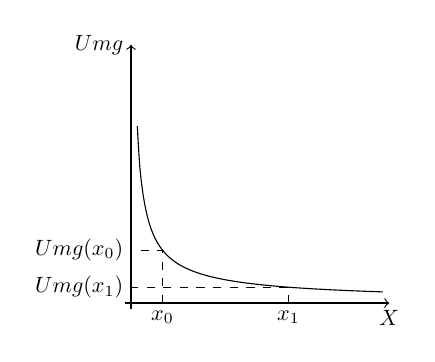
\begin{tikzpicture}[
					scale = 0.8,
					every node/.style = {scale = 0.8},
					declare function = {f(\x)=(1/2)*\x^(-3/4);}
					]

					\draw[->] (0,-0.1) -- (0,4.1) node[left]{$Umg$};
					\draw[->] (-0.1,0) -- (4.1,0) node[below]{$X$};

					\onslide<4->{\draw[dashed] (0.5,0)node[below]{$x_0$} -- (0.5,{f(0.5)}) -- (0,{f(0.5)})node[left]{$Umg(x_0)$};}
					\onslide<5->{\draw[dashed] (2.5,0)node[below]{$x_1$} -- (2.5,{f(2.5)}) -- (0,{f(2.5)})node[left]{$Umg(x_1)$};}

					\draw[samples=200,domain=0.1:4,variable=\x] plot (\x,{f(\x)});
				\end{tikzpicture}
			\end{center}
		\end{column}
	\end{columns}

	\vspace{0.2cm}

	\onslide<6->{Estamos a aproximar o ponto de saciedade! $\rightarrow$ O ponto em que o consumo de um adicional n\~ao aumenta a satisfa\c c\~ao, ou seja o ponto em que $Umg=0$}
\end{frame}

\begin{frame}
	\frametitle{Leis de Gossen}
	\begin{itemize}
		\item \textbf{1\textsuperscript{a} Lei de Gossen:} uma unidade adicional de um bem tem uma utilidade adicional cada vez menor \`a medida que o consumo vai aumentando - a utilidade marginal \'e descrescente!
		\item<2->\textbf{3\textsuperscript{a} Lei de Gossen:} \'e a da escassez, que vem o valor econ\'omico
	\end{itemize}
\end{frame}

\begin{frame}
	\frametitle{Utilidade Marginal}
	A utilidade marginal influencia directamente a disponibilidade a pagar por mais uma unidade de um bem:
	\begin{itemize}
		\item<2->Quanto mais se consome de um bem, menor a utilidade marginal de mais uma unidade, ou
		\item<3-> Menor o valor que o consumidor lhe atribui, portanto, menor a sua disponibilidade a pagar...
	\end{itemize}
	\onslide<3->{\textbf{Pre\c co de reserva:} m\'aximo que o consumidor est\'a disposto a pagar por uma unidade adicional do bem.}
\end{frame}

\begin{frame}
	\frametitle{TMS e Utilidade Marginal}
	Uma Curva de Indiferen\c ca cont\'em todos os cabazes indiferentes a um cabaz $A$, ou seja, todos os cabazes dessa curva t\^em uma tuilidade igual a $U(A)$!

	\vspace{0.2cm}

	Ao longo da curva de indiferen\c ca, alterar $X$ ou $Y$ n\~ao pode alterar $U(A)$, caso contr\'ario n\~ao se estaria ainda na mesma curva...
\end{frame}

\begin{frame}
	\frametitle{TMS e Umg}
	$A\rightarrow C$ redu\c c\~ao de $Y$ \emph{c\ae teris paribus}\\
	$C\rightarrow B$ aumento de $X$ \emph{c\ae teris paribus}
	\begin{center}
		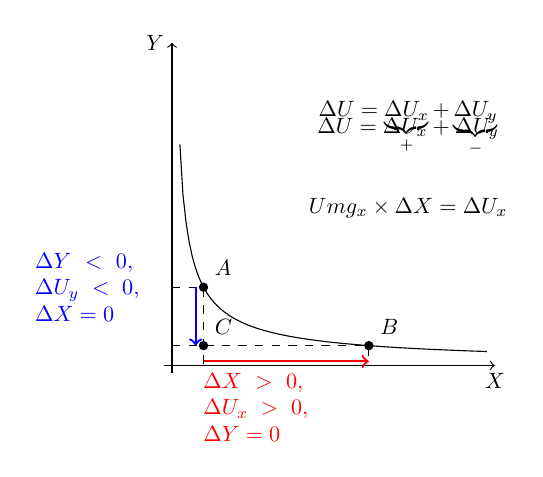
\begin{tikzpicture}[
			scale = 1,
			every node/.style = {scale = 0.8},
			declare function = {f(\x)=(1/2)*\x^(-3/4);}
		]

			\draw[->] (0,-0.1) -- (0,4.1) node[left]{$Y$};
			\draw[->] (-0.1,0) -- (4.1,0) node[below]{$X$};

			\draw[samples=100,domain=0.1:4,variable=\x] plot (\x,{f(\x)});

			\onslide<2->{
				\draw[dashed] (0,{f(0.4)}) -- (0.4,{f(0.4)}) node[circle,fill,inner sep=1.5pt,label=above right:$A$]{} -- (0.4,0);
				\draw[dashed] (0,{f(2.5)}) -- (2.5,{f(2.5)}) node[circle,fill,inner sep=1.5pt,label=above right:$B$]{} -- (2.5,0);
			}
			\onslide<3->{
				\draw (0.4,{f(2.5)}) node[circle,fill,inner sep=1.5pt,label=above right:$C$] {};
			}

			\onslide<4->{
				\draw[->,thick,blue] (0.3,{f(0.4)}) -- (0.3,{f(2.5)});
				\draw (0.3,{f(0.4)}) node[blue,left,text width = 0.2\textwidth] {$\Delta Y<0$, $\Delta U_y < 0$, $\Delta X = 0$};
			}
			
			\onslide<6->{
				\draw[->,thick,red] (0.4,{f(2.5)-0.2}) -- (2.5,{f(2.5)-0.2});
				\draw (0.3,0) node[red,below right,text width = 0.2\textwidth] {$\Delta X>0$, $\Delta U_x > 0$, $\Delta Y = 0$};
			}

			\onslide<7>{
				\draw(3,3) node[]{$\Delta U = \Delta U_x + \Delta U_y$};
			}

			\onslide<8>{
				\draw(3,3) node[]{$\Delta U = \underbrace{\Delta U_x}_{+} + \underbrace{\Delta U_y}_{-}$};
				\draw(3,2) node[]{$Umg_x\times\Delta X = \Delta U_x$};
			}

		\end{tikzpicture}
	\end{center}
\end{frame}

\begin{frame}
	\frametitle{TMS e Utilidade Marginal}
	Ao longo da Curva de Indiferen\c ca, $\Delta U = 0$

	Se $X$ ou $Y$ alterarem a sua quantidade, a altera\c c\~ao em $U$ \'e:
	\begin{align*}
		\onslide<2->{\Delta U &= Umg_x \times \Delta X + Umg_y \times \Delta Y}\\
		\onslide<3->{\Delta U = 0\quad &\Leftrightarrow\quad Umg_x \Delta X = -Umg_y \Delta Y \\
		&\text{ou,}}\\
		\onslide<4->{\frac{\Delta Y}{\Delta X} &= -\frac{Umg_x}{Umg_y}=TMS}
	\end{align*}
\end{frame}

\begin{frame}
	\frametitle{TMS e 1\textsuperscript{a} Lei de Gossen}
	\begin{itemize}
		\item Verific\'amos que $|TMS|$ \'e decrescente \`a medida que $X$ aumenta e $Y$ diminui
		\item<2-> Se $\frac{Umg_x}{Umg_y}=|TMS|$ e dada a 1\textsuperscript{a} Lei de gossen:
	\end{itemize}

	\onslide<2->{
		\begin{align*}
			\left.
			\begin{array}{c}
				\downarrow Y \quad\Rightarrow\quad \uparrow Umg_y\\
				\uparrow X \quad\Rightarrow\quad \downarrow Umg_x\\
			\end{array}\right\}\Rightarrow \quad\downarrow \frac{Umg_x}{Umg_y} = \downarrow TMS
		\end{align*}
	}
\end{frame}

\begin{frame}
	\frametitle{TMS e 1\textsuperscript{a} Lei de Gossen}
	O consumidor $A$ valoriza o bem $Y$ muito mais do que o consumidor $B$

	\begin{columns}
		\begin{column}{0.47\textwidth}
			\begin{center}
				\begin{tikzpicture}[
					scale = 0.8,
					every node/.style = {scale = 0.8},
					declare function = {f(\x)=(1/2)*\x^(-3/4);}
					]

					\draw[->] (0,-0.1) -- (0,4.1) node[left]{$Y$};
					\draw[->] (-0.1,0) -- (4.1,0) node[below]{$X$};

					\onslide<2->{\draw[dashed] (0.5,0)node[below]{$x_0$} -- (0.5,{f(0.5)}) -- (0,{f(0.5)})node[left]{$y_0$};}
					\onslide<3->{\draw[dashed] (2.5,0)node[below]{$x_1$} -- (2.5,{f(2.5)}) -- (0,{f(2.5)})node[left]{$y_1$};}

					\draw[samples=200,domain=0.1:4,variable=\x] plot (\x,{f(\x)});
				\end{tikzpicture}
				Consumidor $A$
			\end{center}
		\end{column}
		\begin{column}{0.47\textwidth}
			\begin{center}
				\begin{tikzpicture}[
					scale = 0.8,
					every node/.style = {scale = 0.8},
					declare function = {f(\x)=(1)*\x^(-1);}
					]

					\draw[->] (0,-0.1) -- (0,4.1) node[left]{$Y$};
					\draw[->] (-0.1,0) -- (4.1,0) node[below]{$X$};

					\onslide<2->{\draw[dashed] (0.5,0)node[below]{$x_0$} -- (0.5,{f(0.5)}) -- (0,{f(0.5)})node[left]{$y_0$};}
					\onslide<3->{\draw[dashed] (2.5,0)node[below]{$x_1$} -- (2.5,{f(2.5)}) -- (0,{f(2.5)})node[left]{$y_1$};}

					\draw[samples=200,domain=0.3:4,variable=\x] plot (\x,{f(\x)});
				\end{tikzpicture}
				Consumidor $B$
			\end{center}
		\end{column}
	\end{columns}
\end{frame}